\documentclass[fontsize=11pt, twoside=false, headings=openany, paper=a4, paper=portrait, twocolumn=false, footinclude=false, headinclude=false, mpinclude=false, pagesize=auto, DIV=12, BCOR=0mm, headlines=1.25, footlines=1.25, parskip=false, headings=small, numbers=enddot, chapterprefix=false, appendixprefix=false, listof=indented, toc=indented, toc=listofnumbered, toc=bibliographynumbered]{scrreprt}% KOMAScript


\usepackage{tum-physics}
\pdftitle{TRM}
\pdfauthor{Michael Labenbacher und Nina Miller}
\pdfsubject{Physics practicum}
\pdfkeywords{TUM, TRM, Physics, Labenbacher, Miller}



\begin{document}
\selectlanguage{naustrian}
\nomatter
\responsible{Michael Labenbacher \&{} Nina Miller}
%\extratitle{Michael Labenbacher}%
%\uppertitleback{Selbstverlag\par Erste Auflage\par Version: \TUMversion{}}%
%\lowertitleback{%
%Satz- und Druckvorstufe: \LaTeX{} mit \KOMAScript{}\par%
%Entwicklungsumgebung: Texmaker 4.5\par%
%Versionsverwaltung: git\par%
%Literaturverzeichnis: JabRef, Bib\LaTeX, %\hologo{biber}
%}%
%\dedication{I would like to dedicate this \dots{}}%
\title{Anfängerpraktikum Teil 1 \\\medskip \LARGE{(Mechanik und Thermodynamik)}}%
\subtitle{Dissoziation und Gefrierpunktserniedrigung}%
\author{Michael Labenbacher \and{} Nina Miller}%
\TUMlogo{\includegraphics[height=0.15\textheight]{TUMlogo.png}}
\TUMphysicslogo{\includegraphics[height=0.15\textheight]{TUMphysicslogo.png}}
\TUMdepartment{Fakultät für Physik}
\TUMuniversity{Technische Universität München}
\TUMpracticaldate{Donnerstag 15.\,März, 2018}
\TUMcoursenumber{3}
\TUMgroupnumber{5}
\TUMteamnumber{14}
%\author{Michael Labenbacher \thanks{Thanks}}%
\maketitle
\frontmatter
%\cleardoublepage\pdfbookmark[0]{\contentsname}{toc}
%\tableofcontents
\mainmatter
%% begin: LaTeX-Einfeuhrung.tex
\chapter{LaTeX-Einführung}
\label{chapter:LaTeX-Einfeuhrung}
Lorem ipsum dolor sit amet, consectetuer adipiscing elit. Aenean commodo ligula eget dolor. Aenean massa. Cum sociis natoque penatibus et magnis dis parturient montes, nascetur ridiculus mus. Donec quam felis, ultricies nec, pellentesque eu, pretium quis, sem.\par\bigskip
Nulla consequat massa quis enim. Donec pede justo, fringilla vel, aliquet nec, vulputate eget, arcu. In enim justo, rhoncus ut, imperdiet a, venenatis vitae, justo. Nullam dictum felis eu pede mollis pretium. Integer tincidunt.
\section{Entwicklung}
\label{section:Entwicklung}
Li Europan lingues es membres del sam familie. Lor separat existentie es un myth. Por scientie, musica, sport etc, litot Europa usa li sam vocabular. Li lingues differe solmen in li grammatica, li pronunciation e li plu commun vocabules.
\subsection{Weiterentwicklung}
\label{subsection:Weiterentwicklung}
\subsubsection{Endstation}
\label{subsubsection:Endstation}
\paragraph{Abschnitt}
\label{paragraph:Abschnitt}
\subparagraph{Unterabschnitt}
\label{subparagraph:Unterabschnitt}
\minisec{Miniüberschrift ohne Referenzierung}
So weit darf es niemals kommen.
\section{Visuelle Darstellung}
\label{section:Visuelle Darstellung}
\begin{figure}%
	\captionsetup{justification=raggedleft, textfont={small,color={orange}}, labelfont={Large,color={\TUMcolor{2}},bf,it}}%
	\includegraphics[scale=0.5,angle=45]{help}%
	\caption{Grafik mit \TUMstyle{1}{\LaTeX{}}-captionsetup in der \TUMstyle{1}{\LaTeX{}}-figure-Umgebung}%
	\label{figure:Grafik mit captionsetup in der figure-Umgebung}%
\end{figure}%
%
{\captionsetup{type=figure,justification=centering}%
	\includegraphics[scale=0.5]{help}%
	\caption{Grafik mit \TUMstyle{1}{\LaTeX{}}-captionsetup- ohne der \TUMstyle{1}{\LaTeX{}}-center-Umgebung}%
	\label{figure:Grafik mit captionsetup ohne der figure-Umgebung}%
}%
%
\begin{figure}%
\captionsetup{justification=centering}%
\subcaptionbox{A\label{subfigure:A}}{\includegraphics[]{help.png}}%
\hfill%
\subcaptionbox{B\label{subfigure:B}}{\includegraphics[]{help.png}}%
\hfill%
\subcaptionbox{C\label{subfigure:C}}{\includegraphics[]{help.png}}%
\hfill%
\subcaptionbox{D\label{subfigure:D}}{\includegraphics[angle=-45]{help.png}}%
\caption{Grafik mit \TUMstyle{1}{\LaTeX{}}-subcaptionbox ohne \TUMstyle{1}{\LaTeX{}}-captionsetup (Standard: komafont)}%
\label{figure:Grafik mit subcaptionbox ohne captionsetup (Standard: komafont)}%
\end{figure}%


\section{Tabellarische Darstellung}
\label{section:Tabellarische Darstellung}
\begin{table}
	\caption{Tabelle mit \TUMstyle{1}{\LaTeX{}}-subtable ohne \TUMstyle{1}{\LaTeX{}}-captionsetup (Standard: komafont)}
	\label{table:Tabelle mit latex-subtable ohne latex-captionsetup (Standard: komafont)}
	\begin{subtable}[b]{\linewidth}
		\caption{Subtable one}
		\label{subtable:Subtable one}
	\begin{tabular}{|r|r|}
		tab & tab2
	\end{tabular}
	\end{subtable}\\
	\begin{subtable}[b]{\linewidth}\centering
		\caption{Subtable two}
		\label{subtable:Subtable two}
	\begin{tabular}{|r|r|}
		tab & tab2
	\end{tabular}
	\end{subtable}
\end{table}

\begin{longtable}{C{0.25\textwidth}Z{p}{0.2\textwidth}{\raggedleft}l}%
	\caption{A long table}\\%
	\toprule	
	f-head & f-head\footnotemark & f-head \\
	\midrule
	\endfirsthead
	\toprule
	head & head & head \\
	\midrule
	\endhead
	\midrule
	foot & foot & foot \\
	\bottomrule
	\endfoot
	\midrule
	l-foot & l-foot & l-foot \\
	\bottomrule
	\endlastfoot
	%% =========================== %%
	\footnotetext{A footnote in the tableentry-firsthead of longtable.\label{footnote:A footnote in the tableentry-firsthead}} a&b\footnote{A footnote in the tableentry-body of longtable.\label{footnote:A footnote in the tableentry-body}} &c\\ a&b&c\\ a&b&c\\ a&b&c\\ a&b&c\\ a&b&c\\ a&b&c\\ a&b&c\\ a&b&c\\ a&b&c\\ a&b&c\\ a&b&c\\ a&b&c\\ a&b&c\\ a&b&c\\ a&b&c\\ a&b&c\\ a&b&c\\ a&b&c\\ a&b&c\\ a&b&c\\ a&b&c\\ a&b&c\\ a&b&c\\ a&b&c\\
\end{longtable}

Nun eine Messwerttabelle von Excel mit input:
\input{tables/test1}


\section{Aufzählungen}
\label{section:Aufzaehlungen}
\begin{enumerate}
\item Ich bin Nummer 1
\item Ich bin Nummer 2
\item Was bin ich?
\end{enumerate}
Oder mit itemize:
\begin{itemize}
\item First
\item[H] Was ist hier falsch :D
\item Third
	\begin{enumerate}
	\item Yeah 1
	\item Yeah 2
	\end{enumerate}
\end{itemize}

\section{Richtiges Referenzieren}
\label{section:Richtiges Referenzieren}
\begin{table}\centering
	\caption{Referenzierungsmöglichkeiten}
	\label{table:Referenzierungsmoeglichkeiten}
	\begin{tabular}{c|c|c|c}%
\TUMstyle{1}{autoref} & 
\TUMstyle{1}{ref} &
self-made-\TUMstyle{1}{ref} &
special \\
%% \autoref{part:Skript}	& 
%% \ref{part:Skript} \\
\autoref{chapter:LaTeX-Einfeuhrung}	 &
\ref{chapter:LaTeX-Einfeuhrung} \\
\autoref{section:Entwicklung} &
\ref{section:Entwicklung} \\
\autoref{table:Referenzierungsmoeglichkeiten} & 
\ref{table:Referenzierungsmoeglichkeiten} \\
\autoref{subtable:Subtable two} & 
\ref{subtable:Subtable two} &
\subtabref{subtable:Subtable two} & 
\subref{subtable:Subtable two}\\
\autoref{figure:Grafik mit subcaptionbox ohne captionsetup (Standard: komafont)} & 
\ref{figure:Grafik mit subcaptionbox ohne captionsetup (Standard: komafont)} \\
\autoref{subfigure:A} & 
\ref{subfigure:A} &
\subfigref{subfigure:A} & 
\subref{subfigure:A}\\
	\end{tabular}
\end{table}
Vom Buch: \cite{AnleitungTRM}, oder siehe Fußnoten: Mit ref: \ref{footnote:A footnote in the tableentry-body}, Mit footref (KomaScript): \footref{footnote:A footnote in the tableentry-firsthead} (Bei Fußnoten kein autoref, da dies nicht unterstütz wird!)


\chapter{Auswertung von Daten}
\label{chapter:Auswertung von Daten}
\section{Visualisierung mit Tikz}
\label{section:Visualisierung mit Tikz}
\begin{figure}\centering
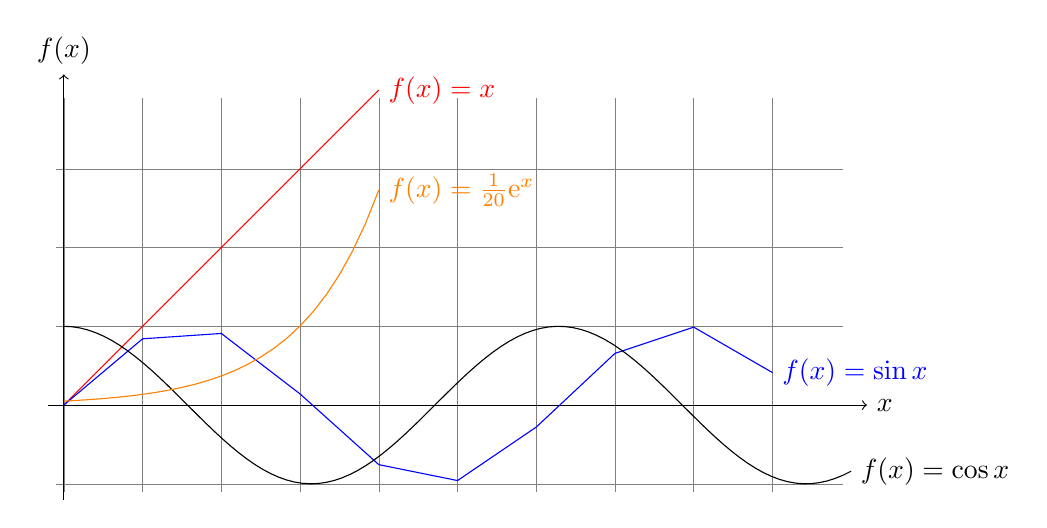
\begin{tikzpicture}[x=10mm,y=10mm]
	\draw[very thin,color=gray] (-0.1,-1.1) grid (9.9,3.9);
    \draw[->] (-0.2,0) -- (10.2,0) node[right] {$x$}; 
    \draw[->] (0,-1.2) -- (0,4.2) node[above] {$f(x)$};
    \draw[color=red]    plot[domain=0:4] (\x,\x)             node[right] {$f(x) =x$}; 
    \draw[color=blue]   plot[domain=0:9,samples=10] (\x,{sin(\x r)})    node[right] {$f(x) = \sin x$}; 
    \draw[color=black]   plot[domain=0:10,samples=100] (\x,{cos(\x r)})    node[right] {$f(x) = \cos x$}; 
    \draw[color=orange] plot[domain=0:4] (\x,{0.05*exp(\x)}) node[right] {$f(x) = \frac{1}{20} \mathrm e^x$};
\end{tikzpicture}
\caption{Plotting a function with Tikz}
\label{figure:Plotting a function with Tikz}
\end{figure}



\begin{figure}\centering
\newcommand{\extrayticklist}{}%
\let\extrayticklist=\empty%
\makeatletter
\foreach \n  in {0,1,2,3,4,5,6}{
	\foreach \m in {1,2,3,4}{
\pgfmathparse{(exp(\n)-exp(\n-1))/5*\m + exp(\n-1)}%
  \ifx\empty\extrayticklist{} \protected@xdef\extrayticklist{\pgfmathresult}%
  \else \protected@xdef\extrayticklist{\extrayticklist,\pgfmathresult}%
  \fi
	}
}
\makeatother
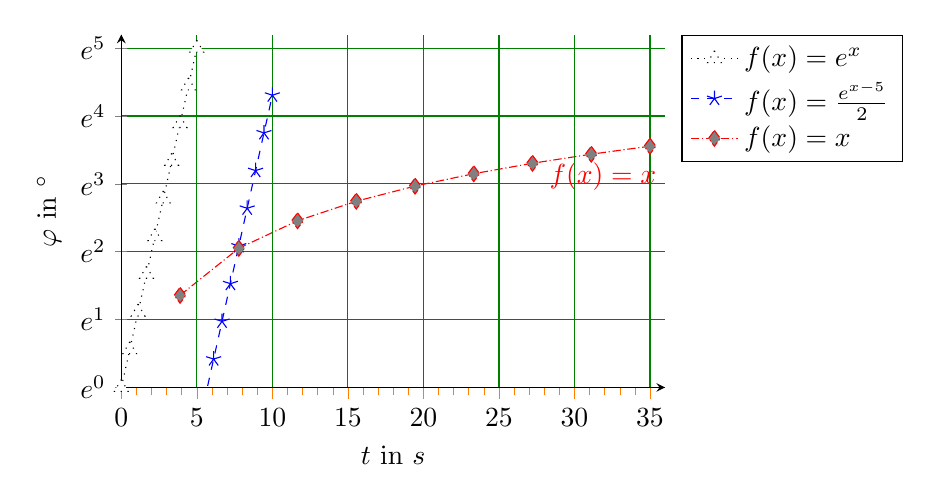
\begin{tikzpicture}[x=10mm,y=10mm]
\pgfmathsetmacro{\expone}{exp(1)}
\begin{axis}[%
xmode=linear,%
ymode=log,%
axis x line = bottom,%
axis y line = left,%
axis on top,%
height=0.5\textwidth,
width=0.7\textwidth,
%log basis ticks={y},
xtick = {0,5,...,35},
minor x tick num=4, 
xtick style = {orange},
xtick align = outside,
grid = major,%
major grid style = {solid, green!50!black},
log basis y={\expone},
log number format basis/.code 2 args={
	$e^{\pgfmathprintnumber{#2}}$},
extra y ticks/.expanded ={\extrayticklist},
every extra y tick/.append style = {% 
	grid = major,%
	major grid style = {dotted, orange!50!black},
   	tick style = {blue},%
    	tick align = outside,% 
},
extra y tick labels={},%
extra x tick style = {% 
	grid = none,%
	%tick style = {orange},%
	%tick align = outside,%
},%
xlabel={$t$ in $s$},
ylabel={$\varphi$ in $^{\circ}$},
xmin=0, xmax=36, ymin=1, ymax={exp(5.2)},
mark size=1mm,
legend pos=outer north east, legend cell align=left,
legend style ={% 
        draw=black, 
        fill=white,},%
]
\addplot[domain=0:5, samples=10, dotted, mark=triangle*, mark options={ fill=white}] {exp(x)};
\addlegendentry{$f(x)=e^{x}$}
\addplot[domain=5:10, samples=10, mark=star, mark options={fill}, dashed, color=blue] {exp(x-5)/2};
\addlegendentry{$f(x)=\frac{e^{x-5}}{2}$}
\addplot[domain=0:35, densely dashdotted, samples=10, color=red, mark=diamond*, mark options={fill=gray}] {x} node[pos=0.9, anchor=north] {$f(x)=x$};
\addlegendentry{$f(x)=x$}
\end{axis}
\end{tikzpicture}
\caption{Plotting a function with axis-environment}
\label{figure:Plotting a function with axis-environment}
\end{figure}


\begin{tikzpicture}[x=10mm,y=10mm]
\begin{axis}[xmode=linear, ymode=linear, axis x line=center, axis y line=center, TUM style 1, xmin=0, xmax=1, ymin=0, ymax=1, grid=both, 
enlarge x limits={rel=0.05,upper},
enlarge y limits={rel=0.05,upper},
xtick distance=0.2, minor x tick num=5,
ytick distance=0.2, minor y tick num=5, 
samples=50, domain=0:1, cycle list name=tumI]
\addplot {x};
\addplot {x/1.2};
\addplot {x/1.4};
\addplot {x/1.6};
\addplot {x/1.8};
\addplot {x/2};
\addplot {x/2.5};
\addplot {x/3};
\addplot {x/5};
\addplot {x/10};
\addplot {x/20};
\end{axis}
\end{tikzpicture}

\begin{figure}
\begin{tikzpicture}
\begin{axis}[xmode=linear, ymode=linear, axis y line=center,
axis x line=center, TUM style 1,
width=\textwidth,
height=0.3\textwidth, 
tick align=center, hide obscured x ticks=true,
ymin=-80, ymax=80, xmin=0, xmax=0.045,
enlarge y limits={abs=19},
enlarge x limits={abs=0.0049,upper},
xtick distance=0.005, minor x tick num=4,
ytick distance=40, minor y tick num=3, 
ymajorgrids, yminorgrids,
ylabel={$u(t)$ in $\mathrm{V}$}, xlabel={$t$ in $\mathrm{s}$}, 
every axis x label/.style={at={(axis description cs:0.95,0.5)}, anchor=south},%
every axis y label/.style={at={(axis description cs:0,1)}, anchor=south},
scaled x ticks={base 10:3},
x tick label style={/pgf/number format/.cd,fixed,precision=1,/tikz/.cd},%
legend cell align=left,
legend style ={% 
	at={(1,1)}, anchor=south east,
        draw=black, 
        fill=white,}%
]%
\addplot [color=RedViolet] table[x index=2,y index=3, col sep = comma] {files/oszi/help/CH1.csv};
\addlegendentry{$u_{1}(t)$}
\addplot [color=ForestGreen] table[x index=2,y index=3, col sep = comma] {files/oszi/help/CH2.csv};
\addlegendentry{$u_{2}(t)$}
\end{axis}
\end{tikzpicture}
\caption{Zeitverläufe der Messgrößen bei $ \alpha = 0 \, ^{\mathrm{ \circ}} $ (B2C mit Energiespeicher)}
\label{figure:Zeitverlaeufe der Messgroessen bei alpha=0 (B2C mit Energiespeicher)}
\end{figure}



\begin{tikzpicture}[baseline]
\begin{axis}[xmode=linear, ymode=linear, axis y line=left,
axis x line=bottom, TUM style 1,
width=0.5\textwidth,
height=0.5\textwidth, 
tick align=outside,
ymin=0, ymax=10, xmin=0, xmax=200,
enlarge y limits={abs=0.9,upper},
enlarge x limits={abs=19,upper},
xtick distance=50, minor x tick num=4,
ytick distance=2, minor y tick num=1, 
xlabel={I/mA},
ylabel={R/$\Omega$}, grid=both]%
%
\addplot+[only marks, /pgfplots/error bars/.cd, y dir = both, y explicit, x dir = both, x explicit] table[y error = dy, x error = dx] {files/help/test.dat};%
%
\end{axis}
\end{tikzpicture}%


\chapter{Mathematik}
\label{chapter:Mathematic}
\begin{align}
\int\limits_{a}^{b} f \left( x \right) \dd{x} &= F(b) - F(a) \\
\pdv[n]{f}{x} &= \dfrac{x^{3}}{3} + \exp \left( -\lambda x \right) + \hypsine \left( x^{3} \right) + \exp \left( - \frac{\mathrm{i}}{x} \right) \notag\\
\sum\limits_{i=1}^{n} a_{n} &= e^{\mathrm{i} \pi } \cdot \sqrt[3]{n}  \xrightarrow{n \to \infty} \infty 
\end{align}

Nun zum Paket siunitx: Man schreibt $a=\SI{5000}{\kilo\gram\metre\per\square\second}$ oder z.\,B. einfach mal etwas so wie $\si{\joule\per\mole\per\kelvin}$, $\si{\kilo\gram_{poly}\squared\per\mole_{cat}\per\hour}$ (für Hochzahlen muss cat als SI-Qualifier erklärt werden in der Preamble!), $\SI{300}{\MHz}$ 



%% end: LaTeX-Einfeuhrung.tex
\chapter{Hello}
\chapter{HelloTwo}\newpage
\chapter{HelloThree}
\section{Sec}
\cite{AnleitungVIS}

\appendix%
\chapter{AppChap1}


\TUMstartlo%
\TUMlistofbibliographies%
\TUMlistoffigures%
\TUMlistoftables%

\backmatter
\end{document}